% Template for ICIP-2018 paper; to be used with:
%          spconf.sty  - ICASSP/ICIP LaTeX style file, and
%          IEEEbib.bst - IEEE bibliography style file.
% --------------------------------------------------------------------------
\documentclass{article}
\usepackage{amsmath,graphicx}

\graphicspath{ {images/} }

% Example definitions.
% --------------------
\def\x{{\mathbf x}}
\def\L{{\cal L}}

% Title.
% ------
\title{Fine Tuning The Rotating Skip List\\Itamar Talmon, Tal Shoef\\
Tel Aviv University}


\begin{document}
%\ninept
%
\maketitle
%
\begin{abstract}
Skip list \cite{C3} is a linked-list-based structure that became an increasingly popular concurrent alternative to search trees due to its logerithmic complexity and local balancing operation. The Rotating skip list \cite{C1} is the fastest concurrent skip list to date. In this paper, we investigate, and try to improve upon, the different heuristics used in the Rotating skip list data structure.
\end{abstract}
%
\section{Introduction}
\label{sec:intro}

\subsection{Concurrent Skip Lists}
\label{ssec:csl}
Skip lists are probabilistic search structures which provide improved execution time bounds compared with straightforward binary search trees yet are much simpler to implement than any guaranteed-$O(\log{n})$ search structure \cite{C3}.
A skip list comprises multiple levels, each of which is a linked list. Every skip-list node is present at the lowest level, and probabilistically present in each higher level up to some maximum level that is chosen independently and randomly for each node. This maximum is selected using a random number generator with
exponential bias: for example, the probability of inserting into level $x$ is often chosen to be $2^{-x}$.
Due to its logerithmic complexity, simplicity and local balancing operation, skip list became an increasingly popular concurrent alternative to search trees and  the default JDK logarithmic concurrent structures (which is an implementation of the lock-free skip list algorithm suggested by Fraser\cite{C4}). Another particularly useful property for parallel skip-list design is that a node can be independently inserted at each level in the list. A node is visible as long as it is linked into the lowest level of the list: insertion at higher levels is necessary only to maintain the property that search time is $O(\log{n})$. This lead to an improved algorithm \cite{C2} that avoids contention hotspots by relying on a maintenance thread to raise, lower and clean-up the towers. This technique lets application threads simply insert an element at the bottom or delete an element by marking it as logically deleted. Yet, untill recently, typical skip list did not exploit multicore platforms as well as trees. This has changed when the Rotating skip list was introduced. The Rotating skip list \cite{C1} combines the rotation of trees and the uncontended nature of skip lists into a multicore-friendly data structure. The core algorithmic novelty is the use of wheels instead of the usual towers that are linked together to speedup traversals.

\subsection{Rotating Skip List Algorithm}
\label{ssec:trsl}

In this section, we present an overview of the rotating skip list key-value store implementation. The rotating skip list differs from traditional skip lists in that it is deterministic and uses wheels, its rotations differ from trees rotations in that they execute in constant time to lower the structure. The resulting algorithm is proven to be linearizable and non-blocking (or lock-free). Refer to \cite{C1} for more details, figures, pseudo code and corectness proofs.

\subsubsection{Key-value store}
\label{ssec:ksv}

Key-value stores offer the basis for indexes to speed up access to data sets. They support the following operations:
\begin{itemize}
	\item  $put(k,v)$ inserts the key-value pair $<k, v>$ and returns $true$ if $k$ is absent, otherwise return $\bot$
	\item  $delete(k)$ removes $k$ and its associated value and returns $true$ if $k$ is present in the store, otherwise return $false$ 
	\item  $get(k)$ returns the value associated with key $k$ if $k$ is present in the store, otherwise return $false$
\end{itemize}

\subsubsection{Structure Memory}
\label{ssec:sm}

Locality is achieved by using a rotating array sub-structure, called the wheel, detailed later in a separate section. The structure is a skip list, denoted $sl$, specified with a set of nodes, including two sentinel nodes. The head node is used as an entry point for all accesses to the data structure, it stores a dummy key that is the lowest of all possible keys. A tail node is used to indicate the end of the data structure, its dummy key is strictly larger than any other possible keys. As in other skip lists, node values are ordered in increasing key order from left to right. The global counter ZERO indicates the index of the first level in the wheels, it is set to 0 intially. The node structure contains multiple fields. It first contains a key-value pair denoted by $<k, v>$. Two special values $v = \bot$ and $v = node$ indicate that the node is logically deleted and physically deleted, respectively. A node is first logically deleted before being physically removed and two logically deleted nodes cannot share the same key $k$. The level represents the level of this node’s wheel, similar to the level of the corresponding tower in a traditional skip list, it indicates that the node keeps track of successors indexed from 0 to level − 1. The succs is the node’s wheel, it stores the successor pointer at each level of the node. next (resp. prev) is a direct pointer to the next (resp. previous) node that contains the smallest key larger than $k$ (resp. the highest key lower than $k$). Hence the skip list nodes are all linked through a doubly linked list. This doubly linked list allows to backtrack among preceding nodes if the traversal ends up at a deleted node. Finally, the marker is a special mark used only during physical removal. 

\subsubsection{Traversal}
\label{ssec:trv}

Each update operation ($put$, $delete$) avoids contention hotspots by localizing the modification to the least contended part of the data structure. All adjustments to the upper levels are sequentially executed by a dedicated maintenance thread, described later, hence allowing a deterministic adjustment of the levels. Any traversal, whether it is for updating or simply searching the structure, is executed from the top of the head node traversing wheels from left to right and levels from top to bottom. Each access looks for the position of some key $k$ in the skip list by starting from the top level of the head down to the bottom level. The $get$ function starts by traversing the structure from the skip list head, namely $sl.head$, till the bottom level. It records the value of ZERO at the beginning of the traversal into a local zero variable, sets its starting point to the $set.head$ before iterating over each level $i$ from the top level of the skip list, which is also the top level of the head $set.head.level - 1$, to zero. Once the $get$ has reached the bottom level, $node$ is actually set to the node with the largest key $k^{'}< k$. If this node is physically deleted, the traversal backtracks among deleted nodes and invokes $help remove$ to notify the background thread of the nodes to be removed. Note that the traversal can thus reach a node that is not linked by any succs pointer but only one next pointer. Then it updates $next$ to the immediate next node ($node.next$). Once the right position at the bottom level indicated by $next.k > k$ is reached, the targeted key $k$ is checked. If it is non logically deleted, the associated value $val$ is returned, otherwise $\bot$ is  returned to indicate that no key $k$ was present in the key-value store. The $put$ function is similar in that it first traverses the structure from top to bottom, backtracks from right to left and help remove deleted nodes. The $put$ may find that the node with the key it looks for is logically deleted, in which case it simply needs to logically insert it by setting its value to the appropriate one using a CAS. if the node is found as non logically deleted, then put is unsuccessful and returns $false$. Finally, if the put did not find the targeted key $k$, it creates a new node node with key $k$ and value $v$ that is linked to next and inserts it physically using a CAS . The reason why nodes are logically deleted before being physically removed is to minimize contention. The delete function marks a node as logically deleted by setting its value to $\bot$. A separate maintenance thread is responsible for traversing the bottom level of the skip list to clean up the deleted nodes as described in later section. The delete executes like the $put$ as it also traverses the structure from top to bottom and backtracks to help remove the deleted nodes. It checks whether a key is absent or if its node is logically or physically deleted in which case it returns $false$. Otherwise, this function logically deletes the node using a CAS to mark it. \textbf{A heuristic helps deciding whether the delete should help removing. This happens only when the ratio of logically deleted nodes over non-logically deleted nodes (as communicated by the background thread) reaches 3 after what it pays off}. Whether it helps physically removing or not, the delete returns $true$ if the node was logically deleted.

\subsubsection{Wheels instead of towers}
\label{ssec:wiot}

The wheel size is adjusted without having to mutate a pointer, simply by over provisioning a static array and using modulo arithmetic to adjust the mutable levels. The modulo arithmetic guarantees that increasing the index past the end of an array wraps around to the beginning of the array. This allows lowering to be done in constant-time by simply increasing the index of the lowest logical level of all the arrays without incurring contention. A global variable ZERO is used to keep track of the current lowest level, and when a lowering occurs the lowest index level is invalidated by incrementing the ZERO variable. This causes other threads to stop traversing the index levels before they reach the previous lowest level of pointers. If ZERO is increased above the length of the array this will not compromise the program since the arrays are accessed with modulo arithmetic. To illustrate how wheels improve locality of reference, consider testing to see if the current node next in the traversal has a key greater than the search key. If the wheels were represented using distinct objects, then $next.k$ would need to be changed to $next.node.k$, reflecting the fact that the key-value information is being stored in a distinct node object from the index next references. This extra layer of indirection can hurt performance of the skip list, especially since this redirects all traversals.

\subsubsection{Background thread}
\label{ssec:bt}

The background (or maintenance) thread executes a loop where it sleeps for 50 microseconds (\textbf{a heuristic parameter}). The maintenance thread raises wheels of non-deleted nodes by calling the $raise bottom level$ function. This raise is compensated with a constant-time lowering specific to the algorithm. This periodic adaptation makes it unnecessary to use the traditional pseudo-random generators as the lowering and raising (the action of increasing the height of a tower) become deterministic. The $lower skiplist$ function discards, in constant-time, the entire bottom level of the skip list by simply changing the ZERO counter used in the modulo arithmetic, without blocking application threads. Note that the $lower skiplist$ is followed by a $cleanup bottom$ level that takes linear time to reclaim the memory of the deleted level, however, all traversals starting after the ZERO increment ignores this level. The $lower skiplist$ function is called, with some heuristic, only if is lowering necessary returns true. \textbf{The chosen heuristic was if there are 10 times more deleted nodes with height greater than 1 than bottom-level nodes}. The $raise bottom level$ also cleans up the skip list by removing the logically deleted nodes. After all logically deleted nodes are discarded, their wheels having been progressively lowered down to a single level, they are garbage collected using an epoch based memory reclamation algorithm discussed later on. The $raise node$ and $raise index level$ simply consist, for each level from bottom to top, of raising each node in the middle of three consecutive non-deleted nodes of the same height. The $help remove$ function called by the $remove$ function or by an application thread removes the deleted nodes. It actually only removes nodes that do not have any wheel successors. Nodes with wheels are removed differently by first lowering their levels. Deleted wheels are simply removed later by the background thread within a $help remove$ during maintenance. Note that at the end of the removal the prev field can be updated without synchronization as it does not have to be set to the immediate previous node.

\subsubsection{Memory reclamation}
\label{ssec:mr}

The memory reclamation of our rotating skip list is based on an epoch based garbage collection algorithm similar to the one used in Fraser’s skip list \cite{C4} with some differences. The garbage collector of Fraser’s skip list is partitioned into sections responsible for managing nodes of a particular skip list level. Partitioning the memory manager like this means that requests to the memory manager regarding different skip list levels do not need to conflict with one another. In contrast, the rotating skip list does no such partitioning of memory management responsibilities, since the rotating skip list uses only one node size for all list elements regardless of their level. This increases the probability of contention in the memory reclamation module when a large number of threads issue memory requests simultaneously.


\subsection{Our Contribution}
\label{ssec:oc}

We examined and extended the following heuristics:

\begin{itemize}
	\item Level Hight Heuristics
	\item Level Delete Heuristics 
	\item Deletion Help Heuristics
	\item Background Thread Sleeping Heuristics
	\item MultiSkipList
\end{itemize}

\hfill \break
Detailed descriptions of the changes made, in addition to the evaluations, are included in the prociding sections of the paper.

\subsection{Code Location}
\label{ssec:cl}
The complete code, including the compiled data strucures and the evaluation script, could be find at \\\texttt{github.com/itamartalmon/synchrobench}.\\\textbf{Note: the code for the Multiple Skip List implementation in located at the \texttt{br\_ts} branch, all the other impementations are located at the \texttt{master} branch}

\section{LEVEL HIGHT HEURISTICS}
\label{sec:lhh}

The skip list maximum level hight is considered to be an important factor to its performence. The reasons for that are three fold:

\begin{itemize}
	\item  A maximum level lower than $\log{N}$, where $N$ is the number of elements in the list, will inevitably hurt the balance properties of the structure and will add to the traversal length
	\item A common cause of contention is the bottle neck at the top layers of the skip list (similar to the root of a tree structure)
	\item Due to its random properties, it is possible (and in fact plausible, in some implementataion) to have unnecessary high levels that will add some overhead work for each traversal
\end{itemize}

In all the implementations we incountered the maximum level of the skip list is bound by some constant (usually the word size of the keys, \textbf{in the case of the rotating skip list - 20}). We examined the effects of choosing the that property in fixed and dynamic ways.

\subsection{Fixed Max Level}
\label{ssec:fml}

Fixing the Max level to a constant is the simplest way to set it. It is a sensible solution where we know the expected size of our structure and expect it to be relativly stable. We wanted to verify that using large max-size hurts performence and benchmarked the original rotating skip list value of 20, against hardcoded value of 40. We tested each implementation for 10 runs, 10 seconds each, with initial size of 524288, key range of 1048576 and update-operations rate (delete / insert) of 20 and 50 percent. \textbf{Note: we also banchmarked using smaller key ranges that did not resulted in any notable difference so their plots were ommited}.

\subsection{Dynamic Max Level}
\label{ssec:dml}

Dynamic Max level is a more sensible solution in cases where we do not know the expected size of the list or that it may changed drastically over time. In our implementation we decided to add a dynamic parameter that stop the list from growing above a certain hight. This parameter is set to be $\log{N}$ in the end of each of the background loop run, where $N$ is the number of non-deleted elements encountered by the background thread. We benchmarked our implementation against the original rotating skip list implementation with the same test properties as above.

\subsubsection{Evaluation}
\label{sssec:ml-evl}

As can be seen on figure 1, the implementation with the hardcoded max level of 40 perfomed worse compare to both the original 20 and the dynamic max-level implementation. Therefore, it seems, that using unnecessary high-max level hurts performence even when raises are deterministic. This could be a result of imbalance caused by the deletes. This seems even more sensible when examining the results of the dynamic max-level compared to the original - in the low update level scenario, the balance of the structure is relativly stable and the overhead of having dynamic max level hurts the performance but in the high updates scenario, the imbalance is higher and hurts the performence more than the dynamic max-level overhead.

\begin{figure}
	\caption{Max Level Heuristics Performence}
	\centering
	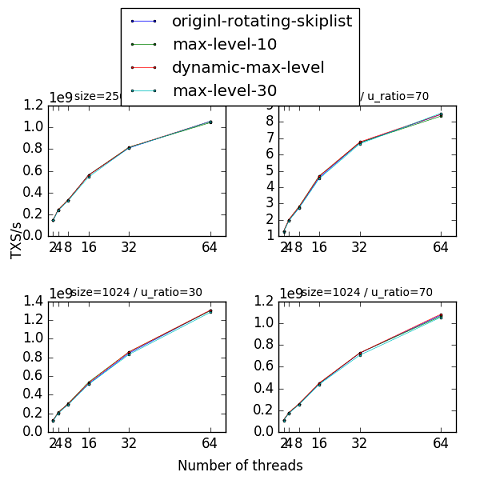
\includegraphics[width=0.6\textwidth]{max-level_plot}
\end{figure}


\section{ROTAION DELETION HEURISTICS}
\label{sec:rdh}

One of the main features of the rotating skip list is the rotation level delete - which efficiantly deletes the first index level at once by increasing the level modulu parameter. The motivation was to balance the effect of deletions on the structure balance (in the rotating skip list - raising nodes indexes cannot cause imbalance due to its deterministic implementation). In the original imlementation, the heuristic used to initiate this action is when the background thread incounter more than 10 times deleted high level nodes (reffered to as tall-deletions) than the number of non-deleted nodes in a single maintenance loop. The authers stated that it might be interesting to investigate different and more dynamic heuristics. We examined the effects of setting different tal-deletion rate constants and implemented our own heurictic (which is based on the size rate between the bottom and the first level and will be described later with more details).

\subsection{Tall-Deletions-Size Rate}
\label{ssec:tds}

Since it does not directly relate to the balance properties of the structure - the idea of conditioning the first layer deletion with the number of the deleted high level nodes might sound a bit strange at first, but since this is the only way that a balanced rotating skip list can become imbalanced, it is a sensible and practical solution (as the background thread is the only one which deletes tall nodes it can easily count them with almost no work or implementation complexity overhead). We wanted to check the way in which the tall-deletion threshold rate parameter influence the skip list performance. We benchmarked the original threshold value of 10 against values of 5, 1 and $1/2$ for 10 runs, 10 seconds each, with initial size of 128 , key range of 256 and update-operations rate (delete / insert) of 30 and 60 percent. In addition, we condacted more tests (ratios of 20 and 70, sizes of 1024 and 512) that did not yield any results that shown difference between the different thresholds and chose not to include their plots.

\subsubsection{Evaluation}
\label{sssec:tds-evl}

As can be seen on figure 2, somewhat surprisingly, using tall-deletion rate thresholds of different orders of magnitude does not improves or compromises the rotating skip list performance under the benchmarked test conditions (which are broader that what was tested in \cite{C1}). This could be a result of the quite extreme condition posed by this heuristic - even for a value of $1/2$ - we so rarely delete more than third of the number of elements in the list and when we do delete, we usualy hurt the performence - as seen for the $1/2$ threshold runs. This suggests that keeping certain, and even relativly large, number of logicaly deleted nodes helps the skip list performance (compared to the situation where those are deleted and others raise for rebealacing). The above makes the effect of this feature on the complexity practicaly negligible.

\begin{figure}
	\caption{Tall Delelted By Size Deletion Performence}
	\centering
	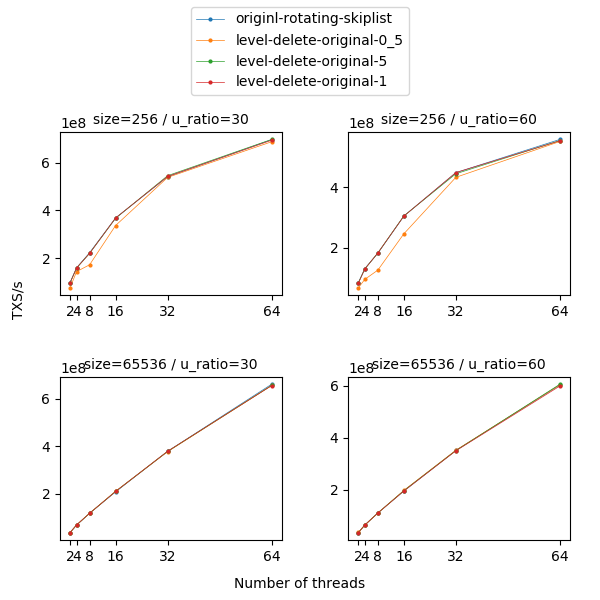
\includegraphics[width=0.6\textwidth]{level-delete-original_plot}
\end{figure}

\subsection{Relative Level Size}
\label{ssec:rls}

The motivation of using the ratio between the first and bottom level came from the clear insight that it is a quality of the rotating skip list that is both easy to obtain (while the backround thread traverse the bottom layer it can just check the nodes level in $O(1)$ time) and a good estimate for the imbalance of the structure. As we expect the first level to be around half the size of the bottom level with thougth that a good threshold for deleting would be $3/4$ as it is half the way between the worst situation, where both level are in similar sizes and the optimal $1/2$ value. We also added a $7/8$ threshold implemtation for the testing in order to better understnad the significance of this feature. We benchmarked the level ratios thresholds of $7/8$ and $3/4$ against the original (tall-deletion ratio threshold) for 10 runs, 10 seconds each, with initial size of 524288, key range of 1048576 and update operations rate (delete / insert) of 20 and 50 percent. As before, we omitted the plots of other test conditions that resulted in similar results. 

\subsubsection{Evaluation}
\label{sssec:rls-evl}

As can be seen on figure 3, the performence of the level ratio delete heuristic was depended on the update-rate test condition. In the low update-rate tests, the original shows the better performance than the level-ratio heuristic implementations. In contrast, in the high update-rate the level-delete heuristic seems to behave better. It is worth to notice that the $3/4$ ratio seems to strike better balance than the $7/*8$. This suggests that the level-ratio heuristic is better estimation of the structure imbalance but it should only be used on a very dynamic situations.

\begin{figure}
	\caption{Levels Ratio Deletion Performence}
	\centering
	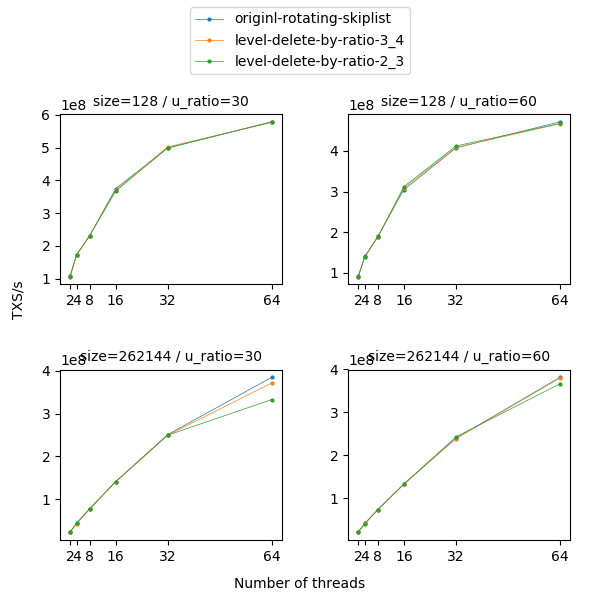
\includegraphics[width=0.6\textwidth]{level-delete-by-ratio_plot}
\end{figure}


\section{DELETION HELP HEURISTICS}
\label{sec:dhh}

In the rotating skip list implementation we first mark a node as logically deleted (to minimize contention) before physically remove it from the list. The background thread is the main thread that is responsible for physically remove nodes but other threads can also help him remove nodes. 

\subsection{Thread-Num-Size Rate}
\label{ssec:tns}

In the original implementation, there is a heuristic that helps deciding whether the delete should help removing. This happens only when the ratio of logically deleted nodes over non-logically deleted nodes (as communicated by the background thread) reaches 3 after what it pays off. We thought that the decision to whether help remove or not should also be taken according to the number of threads. As the number of the threads is bigger the background has much more work to do in order to balance the skip-list structure and maintain the index index levels so help-remove sounds like a good idea. On the other hand, if the number of threads is small, we would rather that there will be more operations happening (add, remove, contains) and the background thread will handle the deletions by itself.
We benchmarked the original heuristic agains ours, (where we take the log of number of threads in consideration when deciding whether the delete should help remove), with initial size of 256 (and 1024), key range of 512 (and 2048) and update operations rate (delete / insert) of 70 (and 90) percent. 

\subsubsection{Evaluation}
\label{sssec:tns-evl}

As We can be seen on figure 4, there are really minor changes between the two heuristics, it seems that as long as the update rate gets higher the performance of our new heuristic that takes in count the number of threads is a bit better than the original, probably because there are more add/delete operations so in case of many threads that are doing many changing list operations (add/remove) it's more critical to enable the help-removing, but anyway, it's not look like something that have significant improvement.

\begin{figure}
	\caption{Help-Remove Performence}
	\centering
	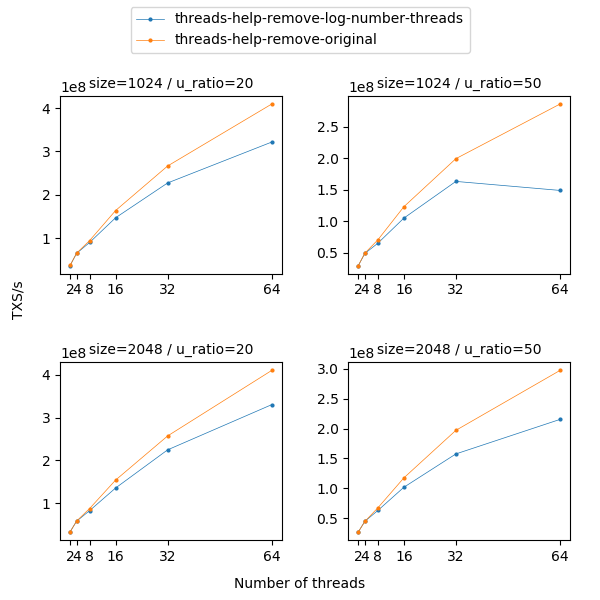
\includegraphics[width=0.6\textwidth]{help-remove_plot}
\end{figure}

\section{BG THREAD SLEEP HEURISTICS}
\label{sec:bts}

The background thread executes a continous loop (until bg\_stop() is called) to maintain index levels. In each iteration the background thread:
\begin{itemize}
	\item traverses the nodes/indexes and for each level from bottom to top it raises each node in the middle of three consecutive non-deleted nodes of the same height 
	\item physically delete logically deleted nodes
	\item remove an entire bottom level of the skip list according to some heuristic
\end{itemize}
\\
The background thread also sleeps for 50 microseconds (a heuristic that is used in the original implementation). We thought it could be interesting to test different heuristics related to sleeping time of the background thread.


\subsection{Thread-Num Rate}
\label{ssec:dsrs1}

Instead of sleep for a constant time (50 microseconds) we thought that the time to sleep should be set according to the number of threads. The reason behind is that as long as we have more threads, there are more operation that is happening, changing the skip list structure, which means, that in order to get good performance we must rebalance the skip-list structure as soon as possible, that's why we decided to decrease the time the background thread sleep (in proportion to the original sleeping time) when the number of thread increases. So when we have a small number of thread, we have less work so the background thread can sleep some more.

\subsection{Sleep double time, Don't sleep at all}
\label{ssec:sdt}

A different heuristic we thought is to make the background thread sleep for double time - 100 ms instead of 50 ms and then canceling the sleep time of the background thread so it won't sleep at all in every second iteration.
We wanted to test if the fact that sometimes the background thread doesn't sleep at all make it better because the skip-list structure should be more balanced.
We benchmarked the original sleep time against the heuristics described in sections 5.1 and 5.2, with initial size of 256 (and 1024), key range of 512 (and 2048) and update operations rate (delete / insert) of 20 (and 50) percent. 

\subsubsection{Evaluation}
\label{sssec:dsrs-evl1}

Evaluation As we can be seen on figure 5, the performance of both of our new heuristics was similar to the one of the original heuristic. Our new heuristics always performed better but it seems to be minor changes. We tested it with different parameters and we got to the conclusion that the sleeping time of the background thread as long as it's not too extreme doesn't affect the performance significantly.

\begin{figure}
	\caption{Background Sleep Time Performence}
	\centering
	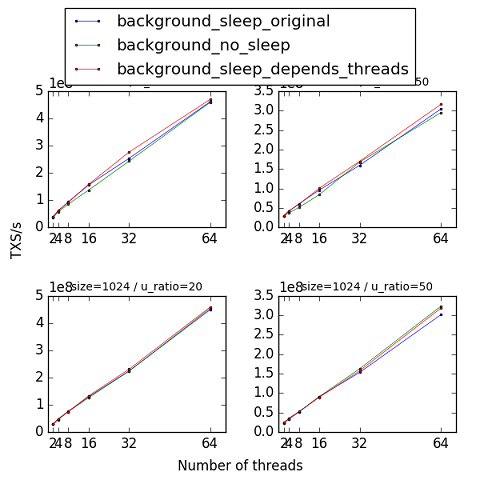
\includegraphics[width=0.6\textwidth]{sleep_plot}
\end{figure}


\section{Multiple Skip Lists}
\label{sec:msl}

The original implementation of the rotating skip list uses one background thread and some worker threads that execute operations like add, remove and contains.
The implementation use only one skiplist that's everybody is working on, along the years the researchers of the skip-list performance tried to diminish contention to get better results.
We thought to go with the same direction, diminish contention, so we decided to use more than one skiplists (in the lines of \cite{C5}). We know that as long as there are many threads, there is still contention, many threads interfering on the same shared data. 


\subsection{Dynamic Number of Skip List}
\label{ssec:dsrs}

We decided that the number of skip lists will be depend on the number of threads because more threads means more contention so our heuristic is to take the number of the skip lists to be half of the number of threads.
We benchmarked the original sleep time against the the multiple skip lists heuristic, with initial size of 128, key range of 256 and update operations rate (delete / insert) of 30 (and 60) percent. 

\subsubsection{Evaluation}
\label{sssec:dsrs-evl}

As can be seen on figure 6, the performance of the multiple skip lists was very similar to the original implementation as long as the number of threads is smaller than 16, what matches our thoughts that our heuristic is good for high contention, many threads interfering to each other. Indeed, when the number of threads increases to 32 and especially 64, we can see that our implementation almost twice as good as the original implementation, which is a significant improvement.

\begin{figure}
	\caption{Multi Skip List Performence}
	\centering
	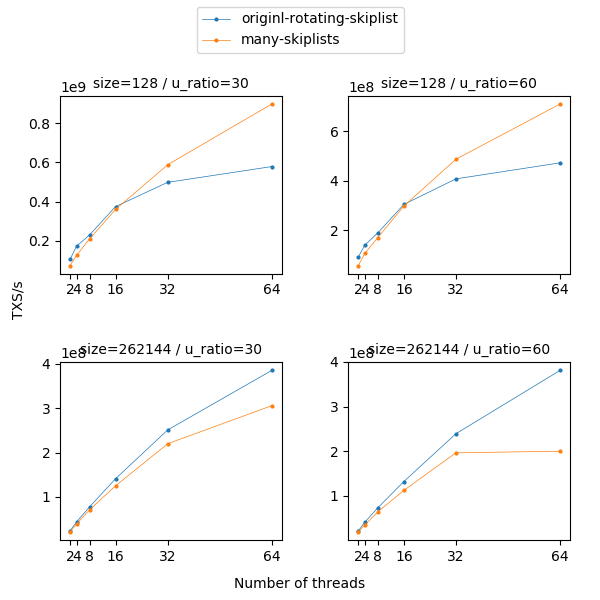
\includegraphics[width=0.6\textwidth]{many-skiplists_plot}
\end{figure}

\section{Experimental Settings}
\label{sec:exp}

We used multicore machine with 8 AMD x86\_64 Opteron(tm) Processor 6376 each have 8 cores that runs at 2.4 GHz. with L1d cache size of 16K, L1i cache size of 64K, L2 cache size of 2048K and L3 cache size of 6144K.

\section{Future Research}
\label{sec:foot}

\subsubsection{Multiple Background Threads}
\label{sssec:mbt}
The amount of maintnance work the background thread need to do is increasing with the size of the list and the number of worker threads and might lead to imbalaced structure in case too much maintnance need to be done. An obvious solution is to incorporate the multiple lists idea with the background thread idea and have few background threads that work on seperate lists and share the work load. This solution keeps the correctness and simplicty of the rotating skip list and will probabily increase performance in cases where a single background thread is over loaded. Perheps the best solution is having worker threads safely 'change into' maintnance threads according to some heuristic. In more general way, it could be interesting designing algorithms that have a dynamic pool of different threads that perform separate tasks in a way that reduces contention.

\subsubsection{Heurictics Based on Action Distribution}
\label{sssec:fr-1}
In some cases, we noticed that some heuristic work better under different update-operations distributions (e.g. 50 \% deletions and inserts). This leads to possible improvment based on keeping some simple approximation of the action distribution inside the skip list itself (e.g. counters for how many inserts/deletes/searchs were performed since the last background loop) and use this estimation to fine tune some thresholds.

\subsubsection{Fine Tuning Probabilistic Skip Lists}
\label{sssec:fr-2}

In this work, we focused only on extending the rotating skip list design but some of the above extensions could be used (with hopefully stronger effects) on probabilistic skip lists implementations. E.g. in a short testing we performed, it seems that the fraser skip list (also used in the JDK) tend to have unnecessary higher levels due to its probabilistic nature and it would be interesting to see how maximum level solutions will effect its performance.


% To start a new column (but not a new page) and help balance the last-page
% column length use \vfill\pagebreak.
% -------------------------------------------------------------------------
%\vfill
%\pagebreak


% References should be produced using the bibtex program from suitable
% BiBTeX files (here: strings, refs, manuals). The IEEEbib.bst bibliography
% style file from IEEE produces unsorted bibliography list.
% -------------------------------------------------------------------------
\bibliographystyle{IEEEbib}
\bibliography{refs}

\end{document}
